% !TeX spellcheck = es_ES
\documentclass[arial,a4paper,print]{article}

\usepackage{amsmath}
\usepackage{amsmath}
\usepackage{amsfonts}
\usepackage{amssymb}
\usepackage{helvet}
\usepackage{lipsum}
\usepackage{multirow}
\usepackage{array}
\usepackage{physics}
\usepackage[version=4]{mhchem}
\usepackage{epsfig}
\usepackage{amssymb}
\usepackage{siunitx}
\usepackage{graphicx}
\usepackage{cancel}
\usepackage{float}
\usepackage{subcaption}
\usepackage[labelfont=sc, font={footnotesize, singlespacing}]{caption}
\usepackage[margin=2cm]{geometry}  

\renewcommand{\familydefault}{\sfdefault}

\usepackage[spanish]{babel}
%opening
\title{Mates: Selectividad 2022}
\author{tomiock}

\begin{document}
\maketitle

Los contenidos consisten en tres grandes bloques (Álgebra Lineal, Geometría y Análisis), pero el e examen tiene tan solo 6 preguntas (de las cuales se escogen 4). 

\section{Álgebra Lineal}
\subsection{Operaciones con matrices}

Las matrices tiene definida una suma, producto y producto por escalar.

Ejemplo de suma de matrices $2\cross2$:
\begin{equation*}
	\begin{pmatrix}
		a_{1} & a_{2} \\
		a_{3} & a_{4}
	\end{pmatrix} +
	\begin{pmatrix}
		b_{1} & b_{2} \\
		b_{3} & b_{4}
	\end{pmatrix} = 
	\begin{pmatrix}
		a_{1} + b_{1} & a_{2} + b_{2} \\
		a_{3} + b_{3} & a_{4} + b_{4}
	\end{pmatrix}
\end{equation*}
Tiene que tener las misma dimensiones. 

En cambio con el producto entre dos matrices, estas no tiene que tener las mismas dimensiones necesariamente. Tal solo el número de filas de una tiene que ser igual que el numero de columnas de la otra y viceversa\footnote{$(m\cross n ) \cdot (n\cross m) \mapsto (m\cross m)$}. Producto entre dos matrices: 
\begin{equation*}
\begin{pmatrix}
	a_{1 1} & \cdots & a_{1 n} \\
	\vdots & \ddots & \vdots \\
	a_{m 1} & \cdots & a_{m n}
\end{pmatrix} 
\begin{pmatrix}
	b_{1 1} & \cdots & b_{1 p} \\
	\vdots & \ddots & \vdots \\
	b_{n 1} & \cdots & b_{n p}
\end{pmatrix} \\
=
\begin{pmatrix}
	a_{11}b_{11}+ \cdots +a_{1n}b_{n1} & \cdots & a_{11}b_{1p}+ \cdots +a_{1n}b_{np} \\
	\vdots & \ddots & \vdots \\
	a_{m1}b_{11}+ \cdots +a_{mn}b_{n1} & \cdots & a_{m1}b_{1p}+ \cdots +a_{mn}b_{np}
\end{pmatrix}
\end{equation*}

O un ejemplo más claro con 2 matrices $(2\cross2)$:
\begin{equation*}
	\begin{pmatrix}
		e & f \\
		g & h
	\end{pmatrix}\begin{pmatrix}
		a & b \\
		c & d
	\end{pmatrix}
	=
	\begin{pmatrix}
		ea + fc & eb + fd\\
		ga + hc & gb + hd
	\end{pmatrix}
\end{equation*}
Se puede ver como es un producto escalar entre vectores que forman columnas y filas:
\begin{figure}[h]
	\centering
	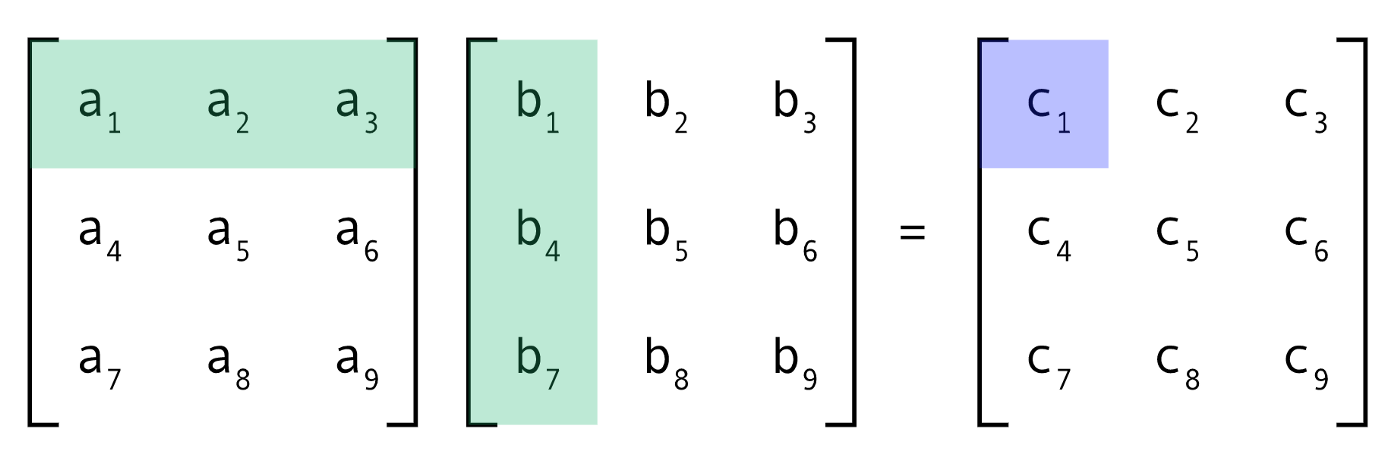
\includegraphics[width=0.5\linewidth]{figures/producto_matrices}
	\caption{Esquema de la multipliación entre dos matrices, el producto escalar de los vectores resaltados en verde dan lugar al escalar marcado en azul. Se coge una fila de la primera matriz y una columna de la segunda. Debido a esto el producto de matrices no es conmutativo $AB\neq BA$.}
	\label{fig:productomatrices}
\end{figure}


Al multiplicar una matriz por un escalar (número), se multiplican todos los elementos de la matriz por ese escalar:
\begin{equation*}
	\begin{pmatrix}
		1 & 4  \\
		3 & 2
	\end{pmatrix}
	=
	\begin{pmatrix}
		5 \times (1) & 5\times (4)  \\
		5\times (3) & 5\times (2) 
	\end{pmatrix}
	=
	\begin{pmatrix}
		5 & 20  \\
		15 & 10
	\end{pmatrix}
\end{equation*}

\subsection{Determinantes}
El determinante es la variación el área/norma que causa una transformación lineal aplicada a una superficie/vector.

El determinantes de una matriz $(2\cross2)$ se calcula con la siguiente regla:
\begin{equation*}
	\det \begin{pmatrix} a & b \\
		c & d \end{pmatrix} = 
	\begin{vmatrix} a & b \\
		c & d \end{vmatrix} = ad - bc
\end{equation*}

Mientras que para una matriz $(3\cross3)$ se puede utilizar la expansión de Laplace\footnote{Muy útil para el cálculo de productos vectoriales entre vectores.}:
\begin{equation*}
	\begin{vmatrix}a&b&c\\ d&e&f\\ g&h&i\end{vmatrix} =
	a\begin{vmatrix}e&f\\ h&i\end{vmatrix} - b\begin{vmatrix}d&f\\ g&i\end{vmatrix} + c\begin{vmatrix}d&e\\ g&h\end{vmatrix}
\end{equation*}
Donde se puede utilizar cualquier columna o fila para expandir la matriz. Dependiendo de la cual, cambia el signo que tiene el determinante. Para un menor $M_{ij}$ el signo que tiene su elemento en la expansión es $(-1)^{i+j}$. Usualmente se da una matriz con un parámetro y se ha de tomar el determinante de esta, resultando en una ecuación de segundo grado normalmente. Es indispensable saber la expansión de Laplace. 

\subsection{Rango de una matriz}

El rango de una matriz es el máximo número de vectores independientes que se pueden sacar de la matriz, ja sean columnas o filas (y no una combinación de las dos). Se puede calcular el rango a partir del orden máximo de los menores no nulos de la matriz (cuando su determinante no es $0$).

Si hay en una matriz hay un menor no nulo de orden $k$ y todos los menores de orden $k+1$ son nulos, entonces el rango de la matriz es $k$. 

Conviene calcular el rango a través de la linealidad de las columnas o filas si se ve inmediatamente. No se pedirá calcular el rango de una matriz de mayor orden que 3.  

\subsection{Matriz inversa}
 $A^{-1}$ es la matriz inversa de $A$ si:
\begin{equation*}
	AA^{-1} = A^{-1}A = I
\end{equation*}
En otras palabras:
\begin{equation*}
	\exists A^{-1} \iff AA^{-1} = A^{-1}A = I
\end{equation*}
Se denomina matriz regular a una matriz que tiene inversa. 

\subsubsection{Cálculo de una matriz inversa}

Se puede calcular mediante la matriz adjunta:
\begin{equation*}
	A^{-1} = \frac{1}{|A|} (A^{\dagger})^{T}
\end{equation*}
Donde $A^{\dagger}$ es la matriz adjunta, definida mediante sus elementos como:
\begin{equation}
	m_{ij} = (-1)^{i+j}M_{ij}
\label{eq:matriz-adjunta}
\end{equation}

Para una matriz $A$ de orden $2$, su adjunta será:
\begin{equation}
	A^{\dagger} = \begin{pmatrix}
		a & b \\ c & d
	\end{pmatrix}^{\dagger} = \begin{pmatrix}
	d & -b \\ -c & a
\end{pmatrix}
\label{eq:2adjunt}
\end{equation}

Y para una matriz $A$ de orden $3$, su adjunta será:
\begin{equation}
	A^{\dagger} = \begin{pmatrix}
		a_{11} & a_{12} & a_{13} \\
		a_{21} & a_{22} & a_{23} \\
		a_{31} & a_{32} & a_{33}
	\end{pmatrix}^{\dagger} = \begin{pmatrix}
	+\begin{vmatrix} a_{22} & a_{23} \\ a_{32} & a_{33} \end{vmatrix} &
	-\begin{vmatrix} a_{21} & a_{23} \\ a_{31} & a_{33} \end{vmatrix} &
	+\begin{vmatrix} a_{21} & a_{22} \\ a_{31} & a_{32} \end{vmatrix} \\
	\\
	-\begin{vmatrix} a_{12} & a_{13} \\ a_{32} & a_{33} \end{vmatrix} &
	+\begin{vmatrix} a_{11} & a_{13} \\ a_{31} & a_{33} \end{vmatrix} &
	-\begin{vmatrix} a_{11} & a_{12} \\ a_{31} & a_{32} \end{vmatrix} \\
	\\
	+\begin{vmatrix} a_{12} & a_{13} \\ a_{22} & a_{23} \end{vmatrix} &
	-\begin{vmatrix} a_{11} & a_{13} \\ a_{21} & a_{23} \end{vmatrix} &
	+\begin{vmatrix} a_{11} & a_{12} \\ a_{21} & a_{22} \end{vmatrix}
\end{pmatrix}
\label{eq:3adjunt}
\end{equation}
Se pueden ver como el elemento de la fila $i$ y la columna $j$ es el menor $M_{ij}$ de la matriz $A$. El término $(-1)^{i+j}$ de la ecuación \ref{eq:matriz-adjunta} indica el signo que se le da a los menor dependiendo de la posición. No hace falta saber la ecuación \ref{eq:matriz-adjunta}, se puede aprender a hacer mecánicamente con la ecuación \ref{eq:3adjunt} y \ref{eq:2adjunt}. 

Haciendo la transpuesta de la adjunta y dividendo los componentes entre el determinante de la matriz original es como se calcula la inversa de esta. 

Sin embargo, usualmente no es necesario utilizar este método porque se puede calcular mediante la resolución de una ecuación matricial, como en este ejemplo:
\begin{align*}
	M^{2} - M -2I = 0\\
	M - I - 2M^{-1} = 0 \\
	- I - 2M^{-1} = - M \\
	M^{-1} = \frac{M-I}{2}
\end{align*}
Siendo $M$ una matriz que cumple $M^{2} - M - 2I = 0$. 


\subsection{Discusión de sistemas}

Los sistemas de ecuaciones se pueden representar mediante matrices: 
\begin{equation*}
	\begin{cases}
		px + y + z = 2\\
		2x + py + p^{2}z = 1\\
		2x + y + z = 2
	\end{cases} \rightarrow \left(\begin{array}{lll|l}
	p & 1 & 1 & 2 \\
	2 & p & p^{2} & 1 \\
	2 & 1 & 1 & 2
\end{array}\right)
\end{equation*}
Donde la última columna representa a que equivale la combinación lineal de los parámetros. Sin embargo siempre que se piensa a discutir el sistema se prescinde de esta columna:
\begin{equation*}
	\left(\begin{array}{lll}
		p & 1 & 1 \\
		2 & p & p^{2} \\
		2 & 1 & 1 
	\end{array}\right)
\end{equation*}

Dependiendo del rango de estas matrices (denominando la primera como matriz ampliada), podemos diferenciar $3$ tipos de sistemas de ecuaciones:
\begin{enumerate}
	\item \textbf{Sistema Compatible Determinado}:\\
	Sistema que tiene un número finito de soluciones. Para un sistema $M$ con una matriz ampliada $M'$, es compatible determinado si el rango de ambas matrices es el orden de $M$: \\
\begin{equation*}
	r(M) = r(M')
\end{equation*}
Si el rango de la matriz es su número de filas se dice que es una matriz '\textit{full rank}' o de rango completo. Para ser un sistema compatible determinado, ambas matrices han de ser de rango completo. 

	\item \textbf{Sistema Compatible Determinado}:\\
	Sistema que tiene infinitas soluciones. Lo es cuando $r(M) = r(M') < \text{orden de $M$}$. Como ejemplo esta el siguiente sistema:
\begin{align*}
	M = \begin{pmatrix}
		2 & 4 & 5 \\
		1 & 3 & 3 \\
		3 & 7 & 8 
	\end{pmatrix} & \qquad M' = \left(\begin{array}{lll|c}
	2 & 4 & 5 & 1 \\
	1 & 3 & 3 & -1 \\
	3 & 7 & 8 & 0 
\end{array}\right)
\end{align*}
Aplicando Gauss podemos ver que: 
\begin{equation*}
	\left(\begin{array}{lll|c}
		2 & 4 & 5 & 1 \\
		1 & 3 & 3 & -1 \\
		3 & 7 & 8 & 0 
	\end{array}\right) \rightarrow \left(\begin{array}{ccc|c}
	2 & 4 & 5 & 1 \\
	0 & -2 & -1 & 3 \\
	0 &-2 & -1 & 3 
\end{array}\right)
\end{equation*}
Y como la matriz tiene dos filas iguales, tiene rango $2$.
Después al mirar  $M$ podemos identificar un menor con determinante no nulo:
\begin{equation*}
	\begin{vmatrix}
		2 & 4 \\ 1 & 3 
	\end{vmatrix} = 2
\end{equation*}
Al tener este menor orden $2$, podemos decir que el rango de la matriz $A$ es igual a $2$.

Al tener la matriz del sistema y su matriz ampliada el mismo rango, siendo esta menor que el orden de la matriz del sistema, se puede decir que el sistema es compatible determinado. 

	\item \textbf{Sistema Incompatible}:\\
Un sistema que no tiene soluciones. Simplemente es cuando $r(M) \neq r(M')$. 
\end{enumerate}

\subsection{Resolución de sistemas}
\subsubsection{Método de Gauss}

Se pueden hacer operaciones de filas en las matrices para de esta manera mirar si sus vectores son dependientes o no. Estas operaciones pueden son las siguientes:
\begin{enumerate}
	\item Permutación de filas (intercambiar de sitio)
	\item Multiplicación de fila por escalar 
	\item Resta/Suma de una fila por otra 
\end{enumerate}

Con estas operaciones se puede conseguir una matriz triangular superior:
\begin{equation*}
	\left(\begin{array}{lcl|c}
		2 & 6 & 9 & 1 \\ 
		0 & -3 & 6 & 1\\ 
		0 & 0 & 7 & 5
	\end{array}\right)
\end{equation*}
A partir de ella se puede resolver el sistema:
\begin{equation*}
	\left(\begin{array}{lcl|c}
		2 & 6 & 9 & 1 \\ 
		0 & -3 & 6 & 1\\ 
		0 & 0 & 7 & 5
	\end{array}\right) \rightarrow \begin{cases}
	2x + 6y + 9z = 1 \\
	-3y + 6z = 1 \\
	7z= 5
\end{cases}
\end{equation*}
 Y entonces $z = \frac57$, y a partir de esto se puede resolver todo el sistema. 

\subsection{Método de Cramer}
Este método no se puede aplicar en sistema Indeterminados. 

Se pueden obtener los parámetros con:
\begin{align*}
	x = \frac{\Delta_{x}}{|M|} \qquad y = \frac{\Delta_{y}}{|M|} \qquad z = \frac{\Delta_{z}}{|M|} 
\end{align*}
 
Para un sistema:
\begin{equation*}
	\begin{cases}
		m_{11}x_{1} + m_{12}x_{2} + m_{13}x_{3} = b_{1} \\
		m_{21}x_{1} + m_{22}x_{2} + m_{23}x_{3} = b_{2} \\
		m_{31}x_{1} + m_{32}x_{2} + m_{33}x_{3} = b_{3} 
	\end{cases}
\end{equation*}
Con su matriz ampliada siendo:
\begin{equation*}
	M' = \left(\begin{array}{lll|l}
			m_{11} & m_{12} & m_{13} & b_{1}\\
			m_{12} & m_{22} & m_{23} & b_{2}\\
			m_{13} & m_{32} & m_{33} & b_{3}
	\end{array}\right)
\end{equation*}

Donde $\Delta_{x}$ es:
\begin{equation*}
	\Delta_{x} = \begin{pmatrix}
		b_{1} & m_{12} & m_{13} \\
		b_{2} & m_{22} & m_{23} \\
		b_{3} & m_{32} & m_{33} 
	\end{pmatrix}
\end{equation*}
Podemos ver como la primera columna a sido sustituida por el vector $\vec{b}$, donde $M\vec{x}=\vec{b}$.

\pagebreak

\section{Geometría}
\subsection{Vectores}
No sé muy bien como explicar que es un vector sin empezar a hablar de mates de la uni, pero lo bueno es que no es necesario saber lo que es. Piensa que es como un número de tres dimensiones que señala un punto en un espacio vectorial\footnote{Tampoco explicaré que es un espacio vectorial porque es chungo hacerlo y no importa mucho. Siempre vamos a trabajar con el mismo espacio, uno de vectores con componentes reales en tres dimensiones.}. 

Por ejemplo esto es un vector:
\begin{equation*}
	\vec{x} = 
	\begin{pmatrix}
		x_{1} \\ x_{2} \\ x_{3}
	\end{pmatrix}
\end{equation*}
Donde sus componentes son $x_{1}, x_{2}, x_{3}$. 

Dado un conjunto de vectores $\{\vec{v_{1}}, \vec{v_{2}}, \cdots, \vec{v_{n}}\}$ una combinación lineal de estos vectores es:
\begin{equation*}
	\lambda_{1}\vec{v_{1}} +  \lambda_{n}\vec{v_{n}} + \cdots + \lambda_{n}\vec{v_{n}} \text{ tal que } \lambda_{1},\lambda_{2}, \cdots, \lambda_{n} \in \mathbb{R}
\end{equation*}

Los vectores $\{\vec{v_{1}}, \vec{v_{2}}, \cdots, \vec{v_{n}}\}$ son linealmente independientes si:
\begin{equation*}
	\lambda_{1}\vec{v_{1}} +  \lambda_{n}\vec{v_{n}} + \cdots + \lambda_{n}\vec{v_{n}} = \vec{0}
\end{equation*}
Donde se puede ver que es verdad si para un conjunto de vectores independientes solo si $\lambda_{1} = \lambda_{2} = \cdots = \lambda_{n} = 0$. 

\subsection{Ecuaciones del plano y la recta}
\subsubsection{Recta}
Es posible definir una recta 3D solo con un punto de posición y un vector director:
\begin{figure}[H]
	\centering
	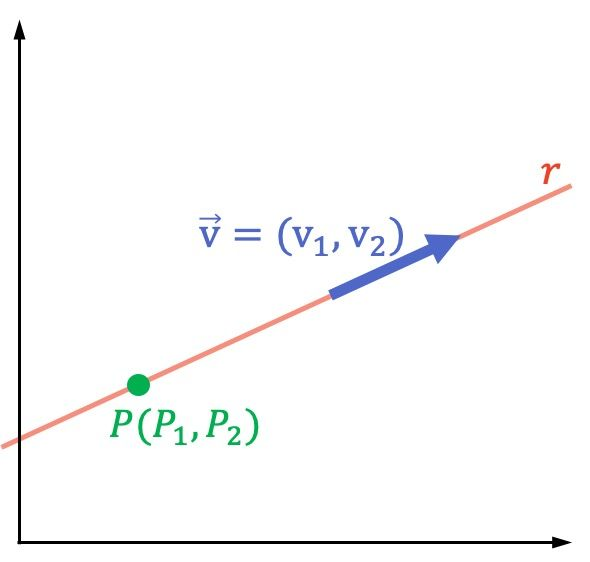
\includegraphics[width=0.3\linewidth]{figures/ecuaciones-de-la-recta}
	\caption{Recta en el espacio con su vector director y punto de posición.}
	\label{fig:ecuaciones-de-la-recta}
\end{figure}

Esto matemáticamente se expresa como (\textbf{Ecuación Vectorial}):
\begin{alignat*}{3}
	\begin{pmatrix} x \\ y \\ z \end{pmatrix} 
	&= \begin{pmatrix} p_{1} \\ p_{2} \\ p_{3} \end{pmatrix} 
	+\lambda\begin{pmatrix} u_{1} \\ u_{2} \\ u_{3} \end{pmatrix} 
\\
\vec{x} &=\vec{p} +\lambda\vec{u}\, , \lambda \in \mathbb{R}
\end{alignat*}

Podemos transformar estos vectores en un sistema de ecuaciones (\textbf{Ecuación Paramétrica}):
\begin{equation*}
	\begin{cases}
		x = x_{0} + \lambda u_{1} \\
		y = y_{0} + \lambda u_{2} \\
		z = z_{0} + \lambda u_{3} 
	\end{cases}
\end{equation*}

Es posible aislar el número $\lambda$ para igualar las ecuaciones (\textbf{Ecuación Continua}):
\begin{equation*}
	\lambda = \frac{x -x_{0}}{u_{1}} = \frac{y -y_{0}}{u_{2}} = \frac{z -z_{0}}{u_{3}}
\end{equation*}

\subsubsection{Plano}
En cambio, un plano se puede definir con un punto de posición y dos vectores:
\begin{figure}[H]
	\centering
	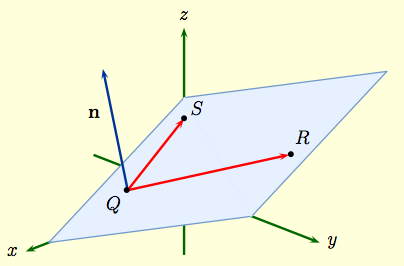
\includegraphics[width=0.4\linewidth]{figures/plane_equation}
	\caption{Se puede ver como el punto de posición $Q$ y los vectores $S$ y $R$, pueden definir el plano. También esta el vector normal $\vec{n}$.}
	\label{fig:planeequation}
\end{figure}

Por lo tanto se puede definir un plano con la siguiente \textbf{Ecuación Vectorial}:
\begin{alignat*}{3}
	\begin{pmatrix} x \\ y \\ z \end{pmatrix} 
	&= \begin{pmatrix} p_{1} \\ p_{2} \\ p_{3} \end{pmatrix} 
	+\lambda\begin{pmatrix} u_{1} \\ u_{2} \\ u_{3} \end{pmatrix} +\mu\begin{pmatrix} v_{1} \\ v_{2} \\ v_{3} \end{pmatrix} 
	\\
	\vec{x} &=\vec{p} +\lambda\vec{u} + \mu\vec{v}\, , \lambda \in \mathbb{R}
\end{alignat*}

La \textbf{Ecuación Paramétrica} sería:
\begin{equation*}
	\begin{cases}
		x = x_{0} + \lambda u_{1} + \mu v_{1} \\
		y = y_{0} + \lambda u_{2} + \mu v_{2} \\
		z = z_{0} + \lambda u_{3} + \mu v_{3} 
	\end{cases}
\end{equation*}

De la ecuación vectorial, sabemos que el vector $\vec{x}-\vec{p}$ es una combinación lineal de los vectores $\vec{u} \text{ i }\vec{v}$. Por lo tanto los vectores $\vec{x}-\vec{p}, \vec{u}, \vec{v}$ son linealmente dependientes y por lo tanto el determinante de la matriz que forma deberá de ser $0$:
\begin{equation*}
	\begin{vmatrix}
		x-x_{0} & u_{1} & v_{1} \\
		y-y_{0} & u_{2} & v_{2} \\
		z-z_{0} & u_{3} & v_{3} 
	\end{vmatrix} = 0
\end{equation*}
Utilizando la expansión de Laplace acabamos en esta ecuación:
\begin{align*}
	(x-x_{0})\begin{vmatrix}
		u_{2} & v_{2} \\ u_{3} & v_{3}
	\end{vmatrix} - (y-y_{0})\begin{vmatrix}
	u_{1} & v_{1} \\ u_{3} & v_{3}
\end{vmatrix} + (z-z_{0}) \begin{vmatrix}
u_{1} & v_{1} \\ u_{2} & v_{2}
\end{vmatrix}
\end{align*} 
Que utilizando un poco de álgebra, podemos acabar con:
\begin{equation*}
	Ax + By + Cz + D = 0
\end{equation*}
Es muy común que en los exámenes se pregunte está ecuación de un plano para definirlo. Se denomina \textbf{Ecuación General} o \textbf{Cartesiana}. 

A partir de esta también se puede definir el vector normal del plano o el vector asociado al plano. Es un vector que es perpendicular al plano. Sus componentes son los parámetros de la ecuación general:
\begin{equation*}
	\vec{n} = \begin{pmatrix}
		A \\ B \\ C
	\end{pmatrix}
\end{equation*}
El número $D$ no forma parte del vector, ya que su función es indicar la posición del plano en el espacio, no su orientación. 

También se puede repasar como definir a una recta a partir de dos planos pero es bastante trivial en mi opinión. Simplemente si te dan dos planos tienes que formar un sistema y resolverlo para un parámetro (tendrá infinitas soluciones claro). 

\pagebreak
\subsection{Posiciones Relativas Planos}

\subsubsection{Planos paralelos}
Para dos ecuaciones generales, los planos son paralelos si:
\begin{equation*}
	\frac{A}{A'} = \frac{B}{B'} = \frac{C}{C'} \neq \frac{D}{D'}
\end{equation*}

No hay una igualdad con $\frac{D}{D'}$ porque en caso de serlo, serían planos coincidentes (el mismo plano):
\begin{equation*}
	\frac{A}{A'} = \frac{B}{B'} = \frac{C}{C'} = \frac{D}{D'}
\end{equation*}

\subsubsection{Planos Secantes}

A partir de dos ecuaciones generales podemos definir un sistema como:
\begin{equation*}
	\begin{cases}
		Ax + By + Cz = -D \\
		A'x + B'y + C'z = -D'
	\end{cases}
\end{equation*}

Al mirar el rango de las matrices si $r(M) = r(M') = 2$, entonces el sistema es compatible indeterminado (infinitas soluciones). Concretamente lo es con un grado de libertad. Estas infinitas soluciones son todos los puntos en la recta. Así también se pueden definir una recta, claro, porque si son secantes, definen una recta.

\subsubsection{Posición Relativa de 3 Planos}

Para tres planos con sus ecuaciones generales:
\begin{align*}
	\pi_1&: Ax + By + Cz = D \\
	\pi_2&: A'x + By' + C'z + D' = 0 \\
	\pi_3&: A''x + B''y + C''z + D'' = 0 \\
\end{align*}

Con las cuales podemos definir una matriz y por lo tanto un sistema:
\begin{equation*}
	\begin{pmatrix}
		A & B & C \\
		A' & B' & C' \\
		A'' & B'' & C'' 
	\end{pmatrix} \begin{pmatrix}
	x \\ y \\ z
\end{pmatrix} = \begin{pmatrix}
	-D \\ -D' \\ -D''
\end{pmatrix}
\end{equation*}

Hay varios casos:
\begin{enumerate}
	\item $r(M) = r(M') = 1$ \\
	Si el rango de ambas matrices es $1$, entonces es un sistema compatible determinado con $2$ grados de libertad, por lo tanto que definen un plano... y entonces pues son el mismo plano (planos coincidentes). 
	
	\item $r(M) = 1$ i $r(M') = 2$\\
	Podemos ver como el sistema es incompatible (sin soluciones) por lo tanto no tiene ningún punto en común y entonces solo pueden ser paralelos o dos puedes ser paralelos y el restante coincidente. Para saber bien su posición, se ha de estudiar si son paralelos entre cada par.
	
	\item $r(M) = r(M') = 2$\\
	El sistema sería compatible indeterminado con un grado de libertad. Si te acuerdas ya hemos hablado de esto, estos planos definen una recta entre dos de ellos o los tres. Para saber exactamente como la definen pues se ha de estudiar si son el mismo plano. 
	
	\item $r(M) = 2$ i $r(M') = 3$\\
	El sistema sería incompatible. Los tres planos no tienen ningún punto en común. Pero claro, dos de ellos si que los pueden tener, definiendo una recta ($r(M) = 2$). El tercer plano puede ser coincidente o paralelo a uno de ellos o definir otra recta. En este caso se dice que los tres planes son secantes de dos a dos. 
	
	\item $r(M) = r(M') = 3$\\
	Realmente este es el caso más fácil, porque los planos coincidirían en un solo punto y ya está :)
\end{enumerate}

\pagebreak
\subsection{Posición Relativa entre Plano y Recta}

Para una recta definida como la interjección entre dos planos:
\begin{equation*}
	\begin{cases}
		Ax + By + Cz + D = 0 \\
		A'x + B'y + C'z + D' = 0 
	\end{cases}
\end{equation*}

Y un plano definido como su ecuación general ($ A''x + B''y + C''z + D'' = 0 $).

Es posible crear el siguiente sistema:
\begin{equation*}
	\begin{cases}
		Ax + By + Cz = D \\
		A'x + B'y + C'z = D' \\
		A''x + B''y + C''z = D'' \\
	\end{cases}
\end{equation*}
A través del cual podemos ver diversos casos:
\begin{enumerate}
	\item $r(M) = r(M') = 2$\\
	El sistema sería compatible indeterminado, es decir, que hay infinitas soluciones. La única posición que puede cumplir esto es que la recta forme parte del plano. 
	
	\item $r(M) = 2$ i $r(M') = 3$\\
	El sistema sería incompatible, por lo tanto la recta únicamente puede ser paralela al plano.
	
	\item $r(M) = r(M') = 3$\\
	Simplemente la recta cruza el plano en un punto :)
	
\end{enumerate}

\subsection{Producto Escalar}
El producto escalar entre dos vectores:
\begin{equation*}
	\vec{a} \cdot \vec{b} = a_{1}b_{1} + a_{2}b_{2} + a_{3}b_{3}
\end{equation*}
Se puede utilizar para obtener información ja que también es definido como:
\begin{equation*}
	\vec{a} \cdot \vec{b} = \norm{a}\norm{b}\cos \theta
\end{equation*}
Donde $\theta$ es el ángulo entre los dos vectores. 

Por lo tanto para $\theta = \frac{\pi}{2}$ los vectores serían perpendiculares y su producto escalar sería igual a $0$, ya que $\cos\frac{\pi}{2} = 0$.

\subsection{Perpendicularidad i Ángulos}

Utilizar este el producto escalar en vectores asociados a un plano, nos puede decir si estos planos son perpendiculares o no, por ejemplo. 

También cuando hablamos de un plano y una recta, esos son perpendiculares si el vector director de la recta y el vector asociado son linealmente dependientes. 

Por último dos rectas son perpendiculares cuando sus vectores directores también lo son. 

Al igual que podemos determinar la perpendicularidad entre dos objectos, también lo podemos hacer con sus ángulos, utilizando también el producto escalar (con el coseno que está en su definición). 

\subsection{Producto Vectorial}
El producto vectorial es muy útil ya que a partir de él se puede 



\section{Análisis}

\end{document}